\documentclass{beamer}
%
% Choose how your presentation looks.
%
% For more themes, color themes and font themes, see:
% http://deic.uab.es/~iblanes/beamer_gallery/index_by_theme.html
%
\mode<presentation>
{
  \usetheme{default}      % or try Darmstadt, Madrid, Warsaw, ...
  \usecolortheme{default} % or try albatross, beaver, crane, ...
  \usefonttheme{default}  % or try serif, structurebold, ...
  \setbeamertemplate{navigation symbols}{}
  \setbeamertemplate{caption}[numbered]
} 

\usepackage[english]{babel}
\usepackage[utf8x]{inputenc}

\title[Your Short Title]{Noise evaluation and reduction}
\author{Hoang Duc Viet}
\institute{ICT Lab}
\date{\today}

\usepackage{subfigure}
\usepackage{graphicx}



\begin{document}

\begin{frame}
  \titlepage
\end{frame}

% Uncomment these lines for an automatically generated outline.
%\begin{frame}{Outline}
%  \tableofcontents
%\end{frame}

\section{Introduction}

\begin{frame}{Introduction}

%Denoising is considered as one of the major issues in image processing.
%The noise in an image can be due to camera sensors, atmospheric conditions or transmission through a medium. Denoising has its root in wide range of applications. %such as segmentation, recognition, classification etc.

\begin{itemize}
  \item Problem
  
  \
  
  \item Solution
  
  \
  
  \item Evaluation
  
  \
  
  \item Results and Discussion

\
 
  \item Conclusion
\end{itemize}

%\vskip 1cm

%\begin{block}{Examples}
%Some examples of commonly used commands and features are included, to help you get started.
%\end{block}

\end{frame}

\section{Some \LaTeX{} Examples}

\subsection{Noise}

\begin{frame}{Problem}

%\textbf{Definition}

%\vspace{0.5cm}

\begin{itemize}



\item Noise:

An unwanted component of the image which can
be additive or multiplicative.
%Noise is the cause of errors from image when in pixel values that do not reflect the true intensities of the real scene.

\vspace{7mm}

\item Denoise:

Popular solution for photography or remove noise in images processing.



\end{itemize}




% Commands to include a figure:
%\begin{figure}
%\includegraphics[width=\textwidth]{your-figure's-file-name}
%\caption{\label{fig:your-figure}Caption goes here.}
%\end{figure}

%\begin{table}
%\centering
%\begin{tabular}{l|r}
%Item & Quantity \\\hline
%Widgets & 42 \\
%Gadgets & 13
%\end{tabular}
%\caption{\label{tab:widgets}An example table.}
%\end{table}

\end{frame}

\subsection{Type of noise}

\begin{frame}{Type of noise}
%\textbf{Definition}

%\vspace{0.5cm}

\begin{itemize}
	\item Salt and Pepper Noise
	


	
	\
	
	\item  Gaussian Noise
	
%	Maybe the most common image noise
	
	\
	
	\item Quantization Noise
	
    \
    
    \item Speckle Noise


\end{itemize}

\end{frame}


\subsection{Original Image}
\begin{frame}{Original Image}

\vspace{1cm}
\begin{center}
%	\includegraphics{}

   % \centering 
    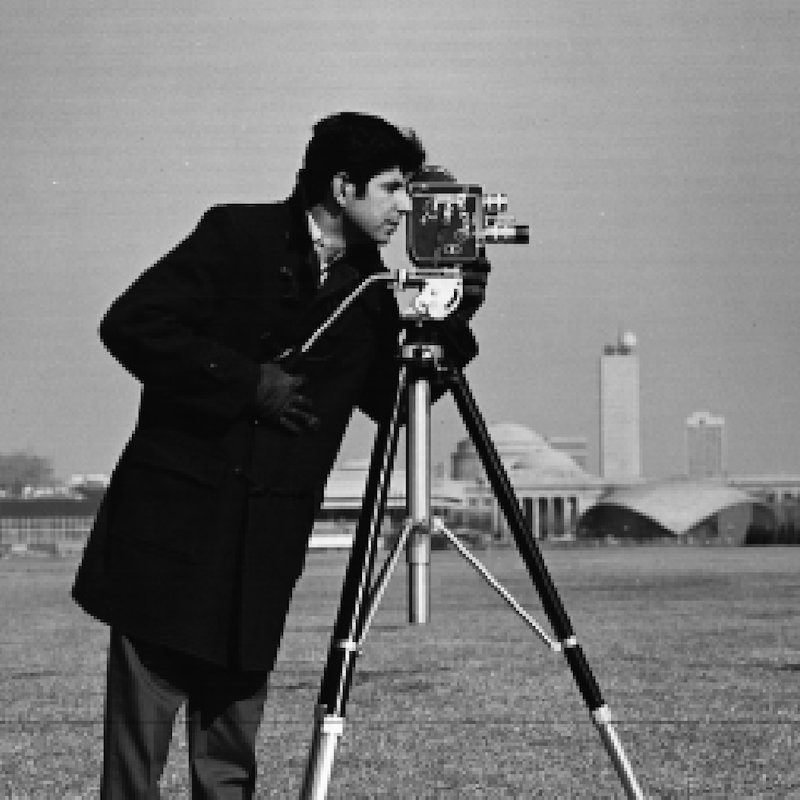
\includegraphics[width=0.4\columnwidth]{images/salt_pepper_origin.jpg}
   % 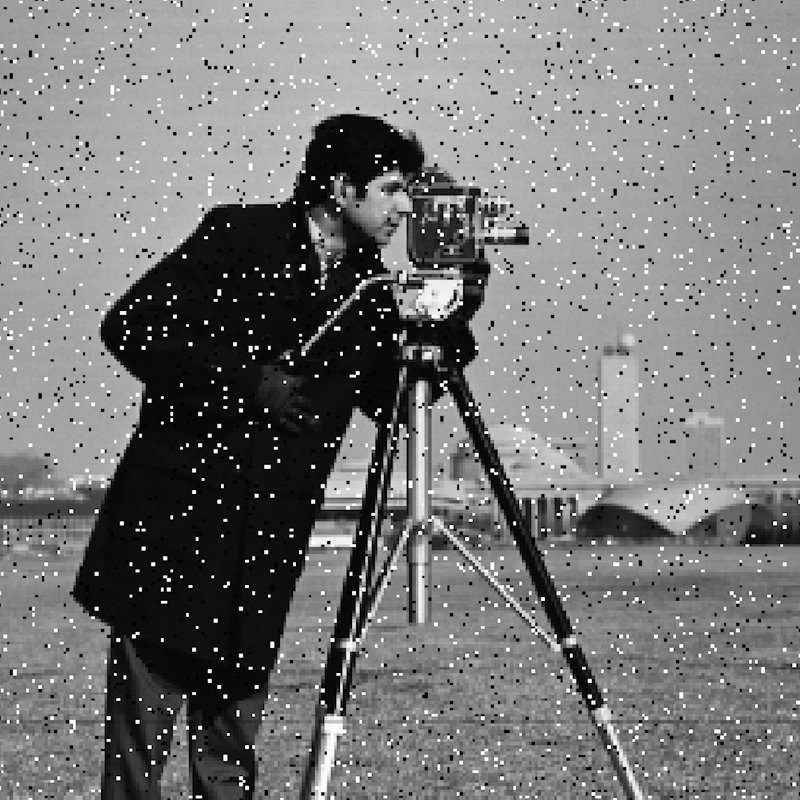
\includegraphics[width=0.4\columnwidth]{images/salt_pepper_noise.jpg}
	
	Original Image



\end{center}

\end{frame}

\subsection{Noise}
\begin{frame}{Noise}

%\vspace{1cm}
%\begin{center}

   % 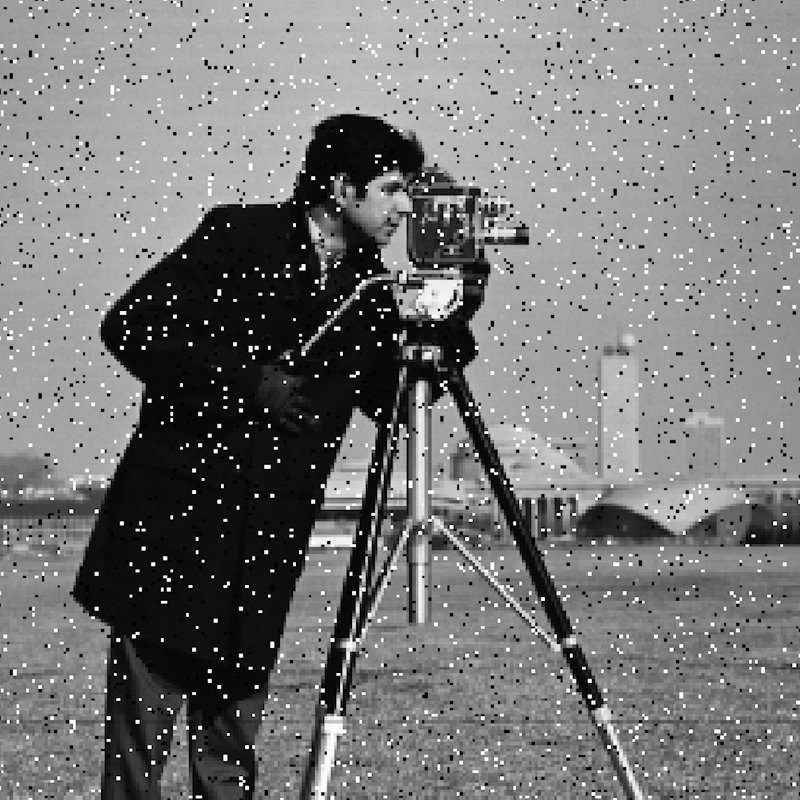
\includegraphics[width=0.27\columnwidth, height=8\baselineskip]{images/salt_pepper_noise.jpg}
    %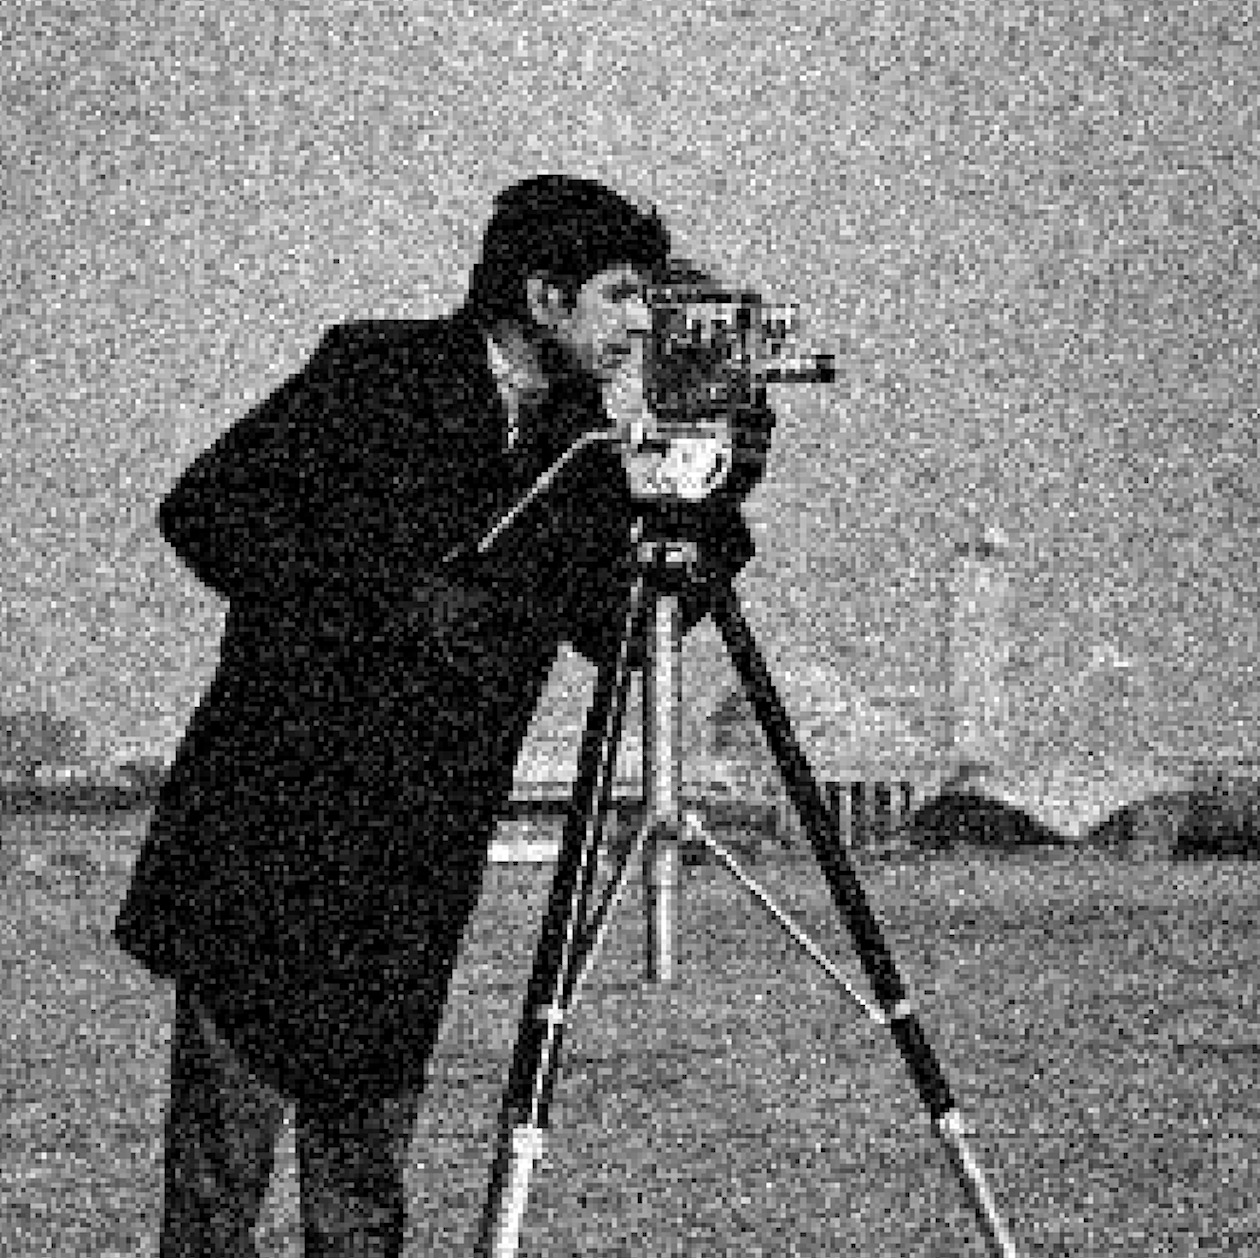
\includegraphics[width=0.27\columnwidth,  height=8\baselineskip]{images/gaussian_noise.jpg}
    %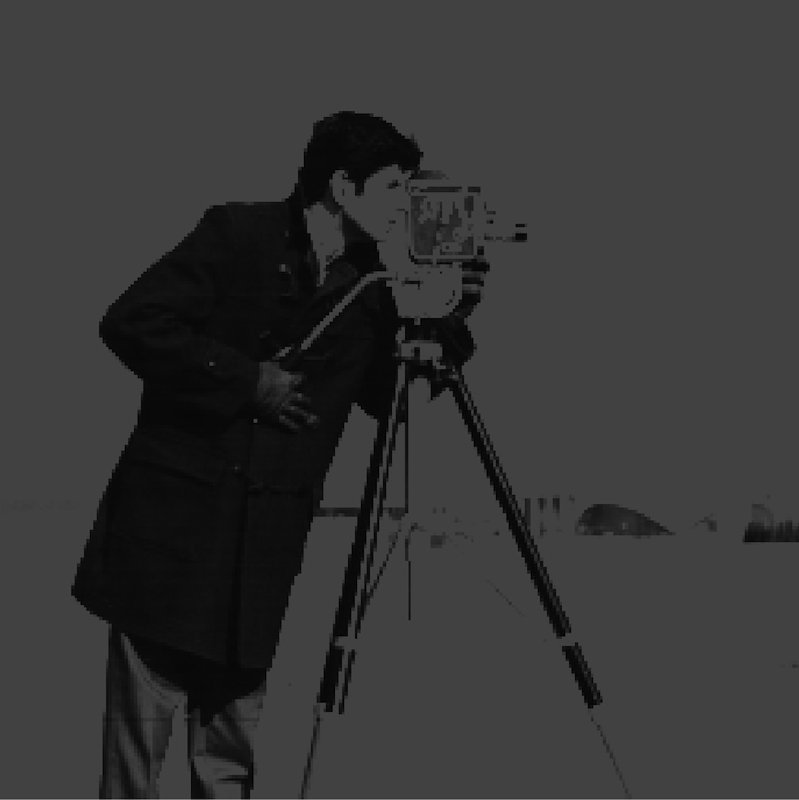
\includegraphics[width=0.27\columnwidth,  height=8\baselineskip]{images/quantization_noise.jpg}
    %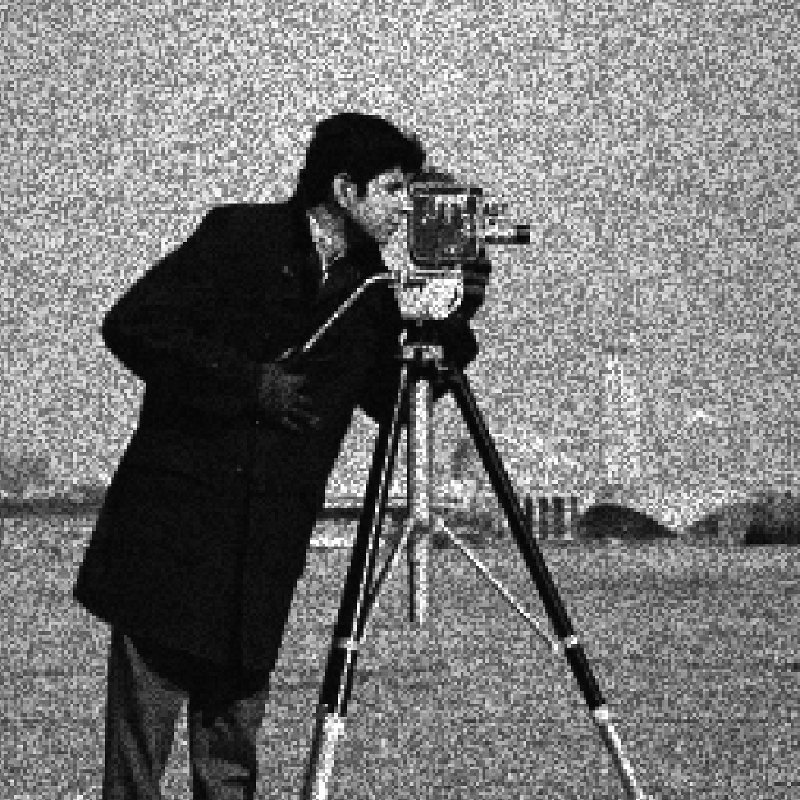
\includegraphics[width=0.27\columnwidth,  height=8\baselineskip]{images/speckle_noise.jpg}
    
    \begin{figure}
    \centering  
    \subfigure[Salt and Pepper]{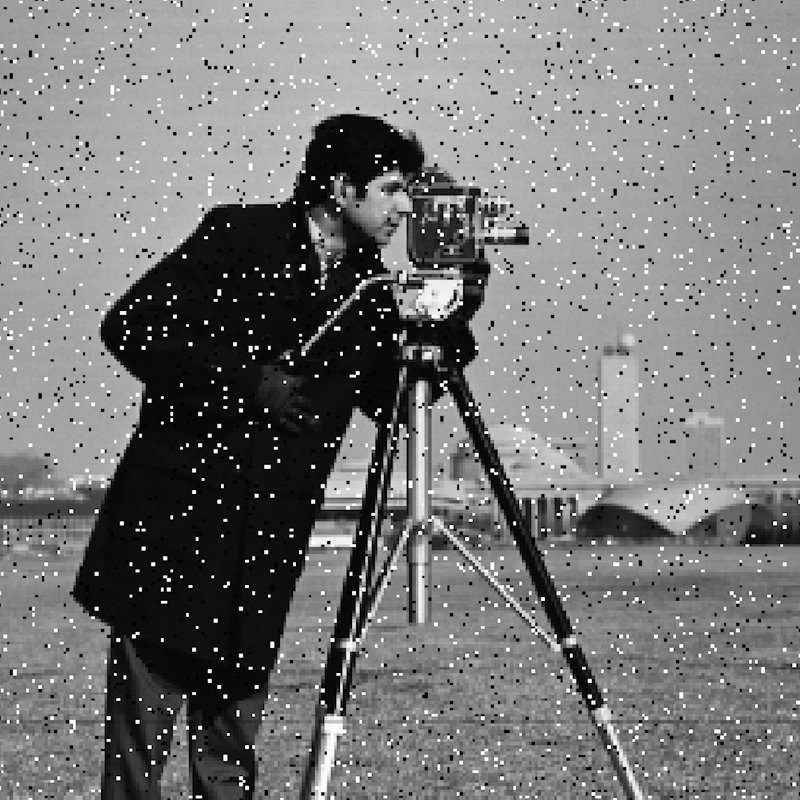
\includegraphics[width=0.4\linewidth, height=3.2cm]{images/salt_pepper_noise.jpg}}
    \subfigure[Gaussian]{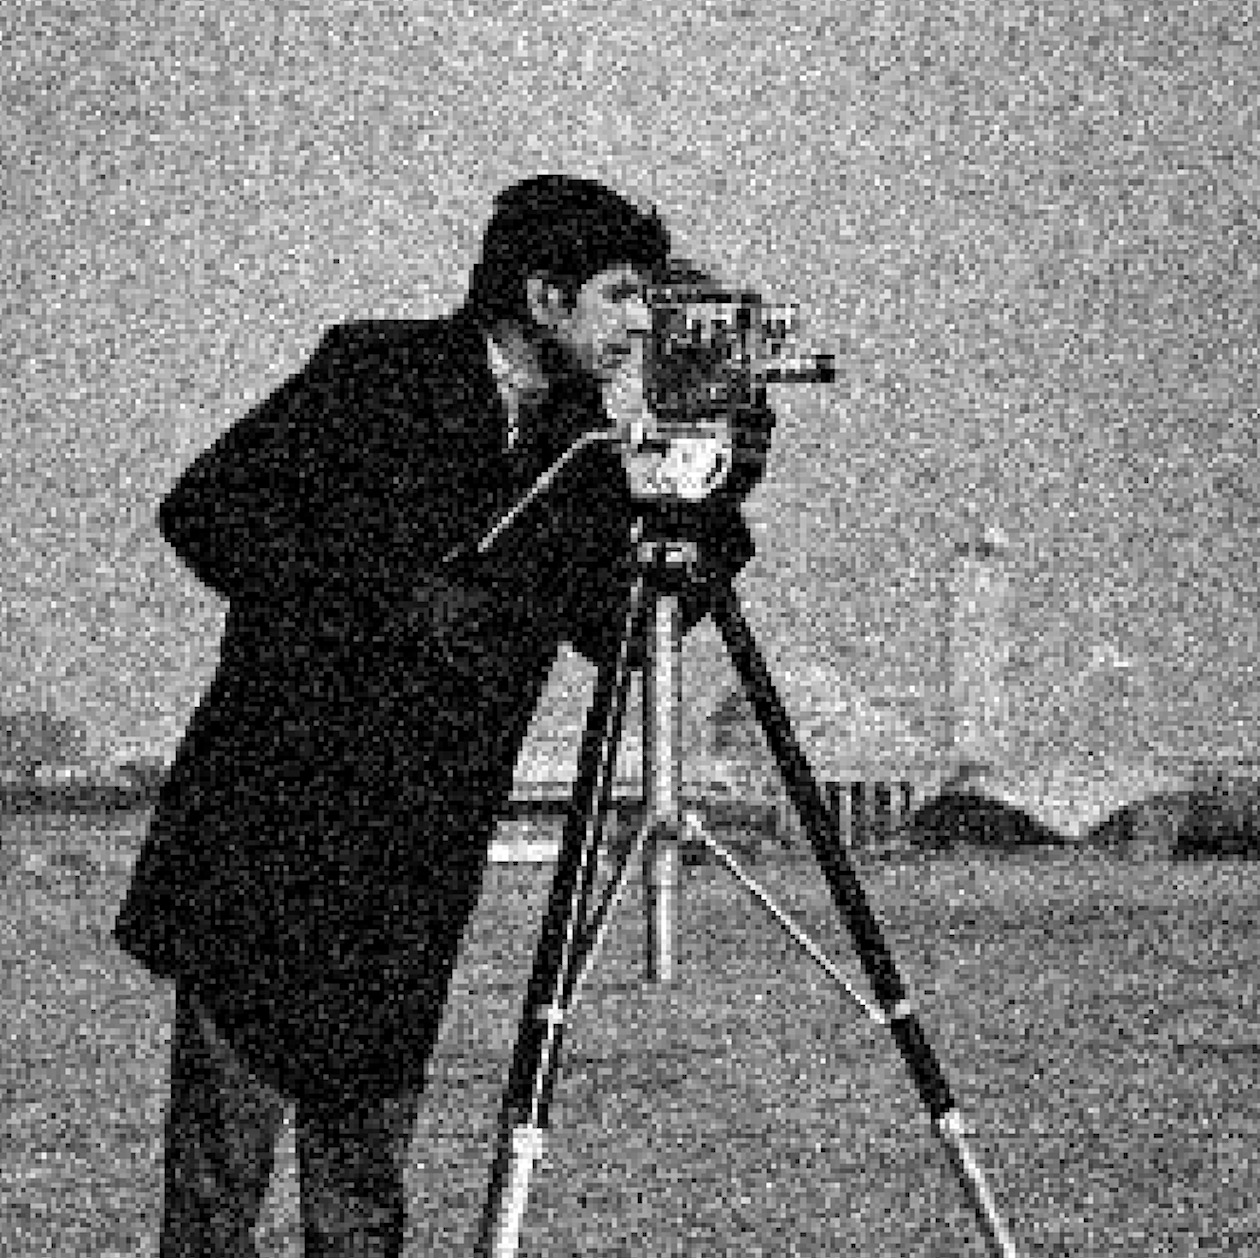
\includegraphics[width=0.4\linewidth, height=3.2cm]{images/gaussian_noise.jpg}}
    \subfigure[Quantization]{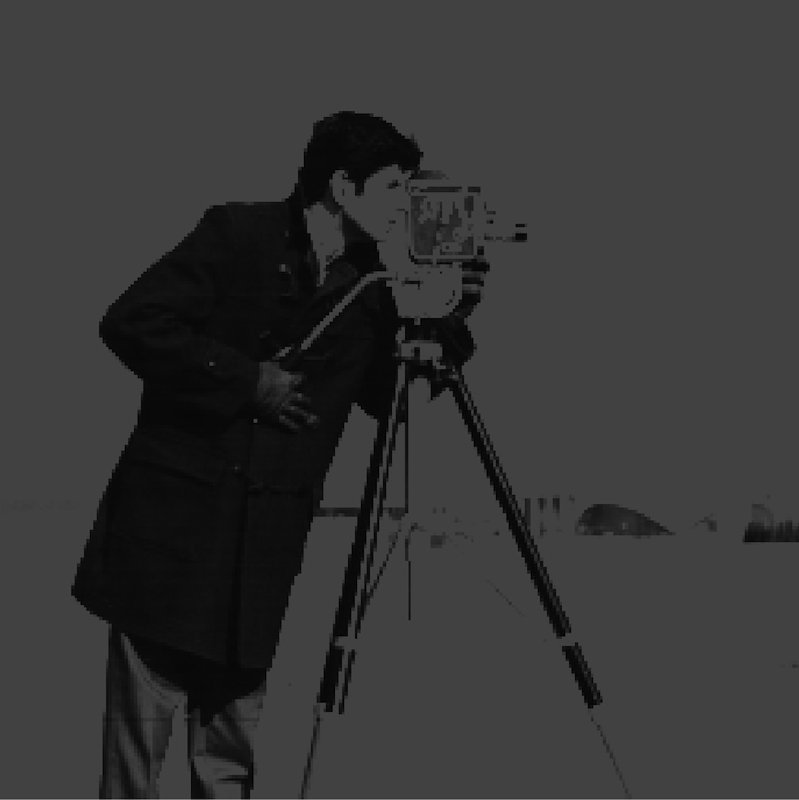
\includegraphics[width=0.4\linewidth, height=3.2cm]{images/quantization_noise.jpg}}
    \subfigure[Speckle]{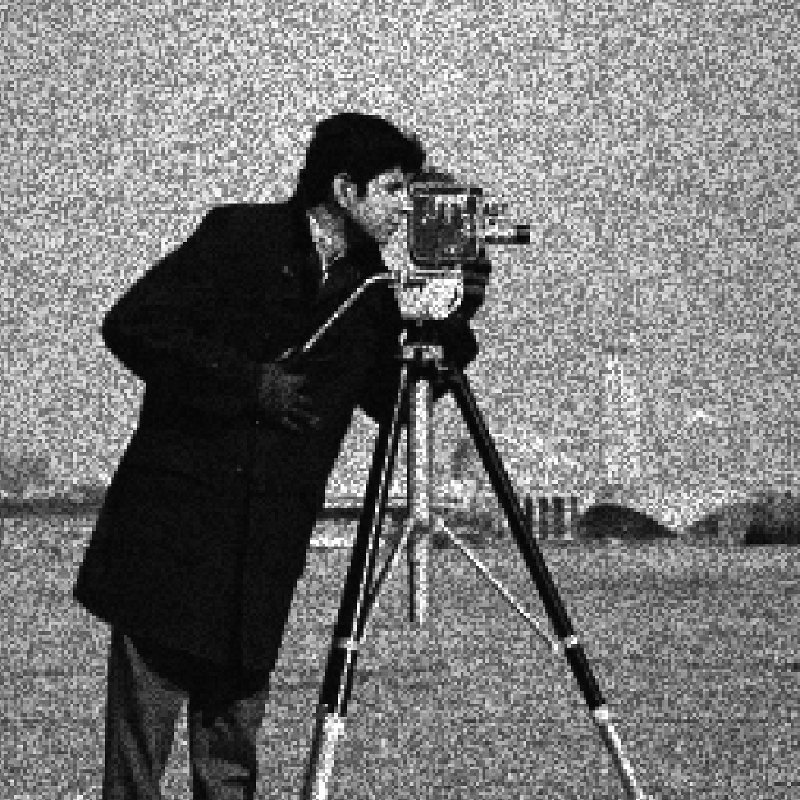
\includegraphics[width=0.4\linewidth, height=3.2cm]{images/speckle_noise.jpg}}
    
    \end{figure}
    
    
    
    
    
   % 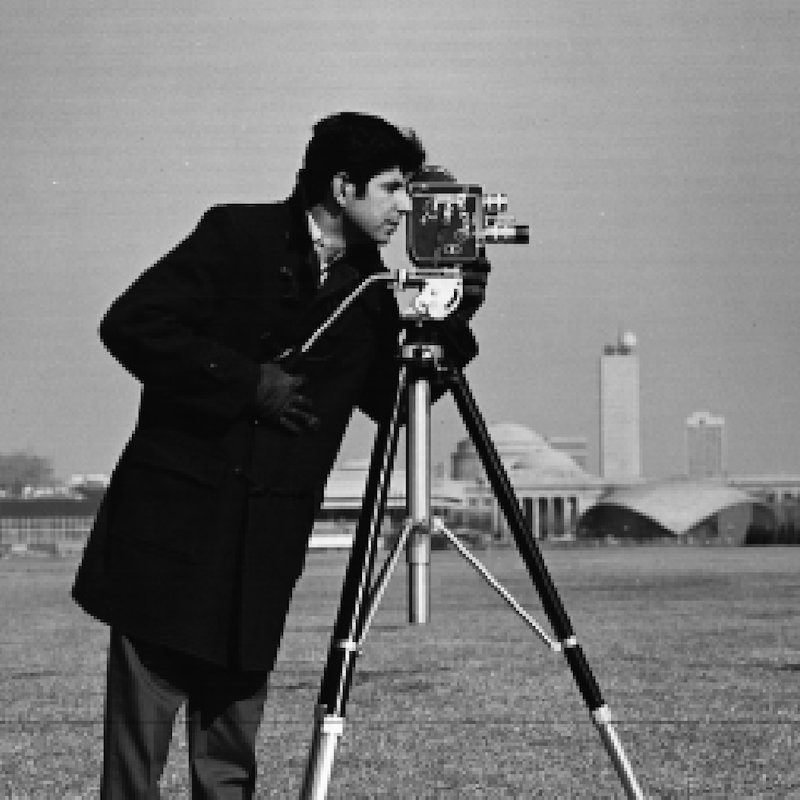
\includegraphics[width=0.4\columnwidth]{images/salt_pepper_origin.jpg}
    %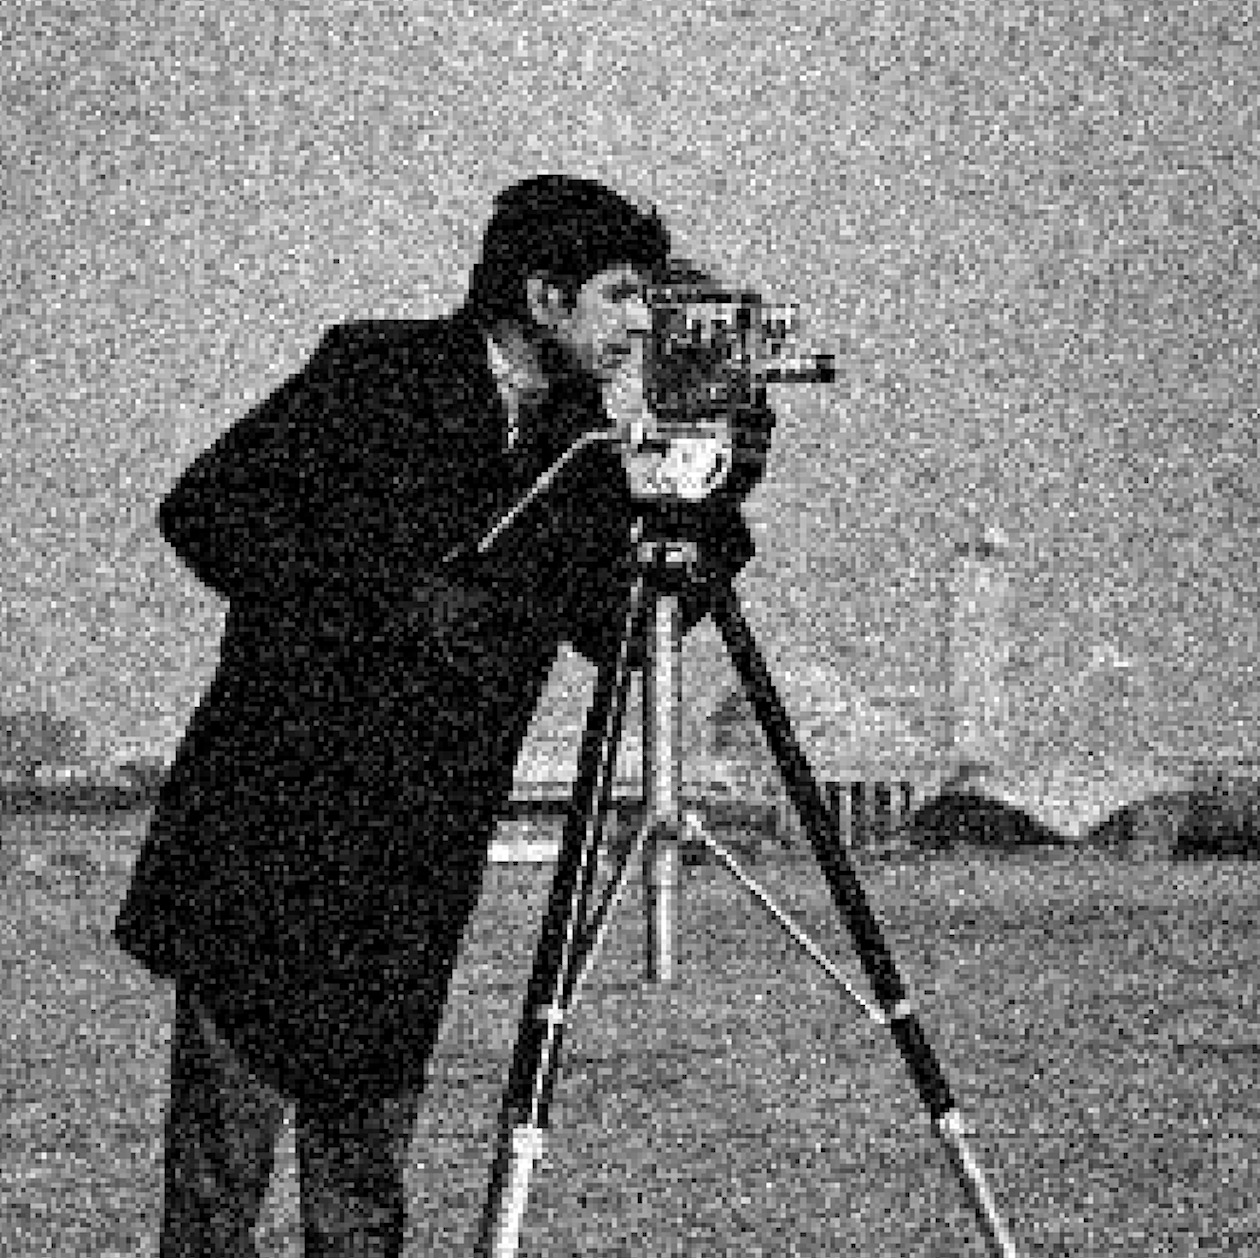
\includegraphics[width=0.4\columnwidth]{images/gaussian_noise.jpg}
	
	%Original image (left column) and gaussian noise (right column).
	


%\end{center}
\end{frame}

%\subsection{Quantization Noise}
%\begin{frame}{Quantization Noise(Uniform Noise)}

%\vspace{1cm}
%\begin{center}
%	  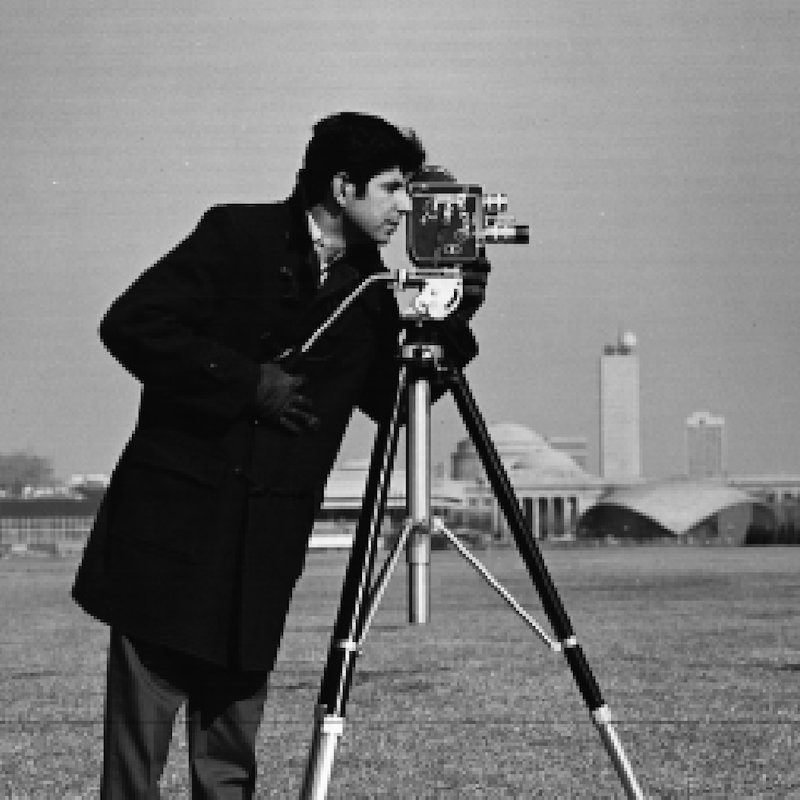
\includegraphics[width=0.4\columnwidth]{images/salt_pepper_origin.jpg}
	  %  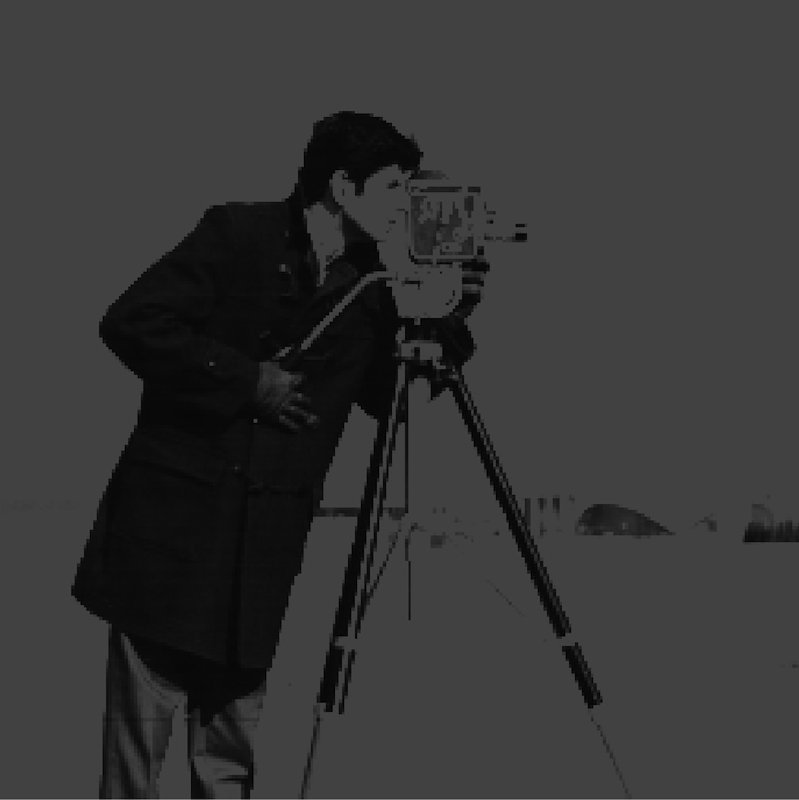
\includegraphics[width=0.4\columnwidth]{images/quantization_noise.jpg}
		
	%	Original image (left column) and quantized image to 6 bits (right column).
	


%\end{center}
%\end{frame}
%\subsection{Speckle Noise}
%\begin{frame}{Speckle Noise(Multiplicative Noise)}
%\begin{center}
 % 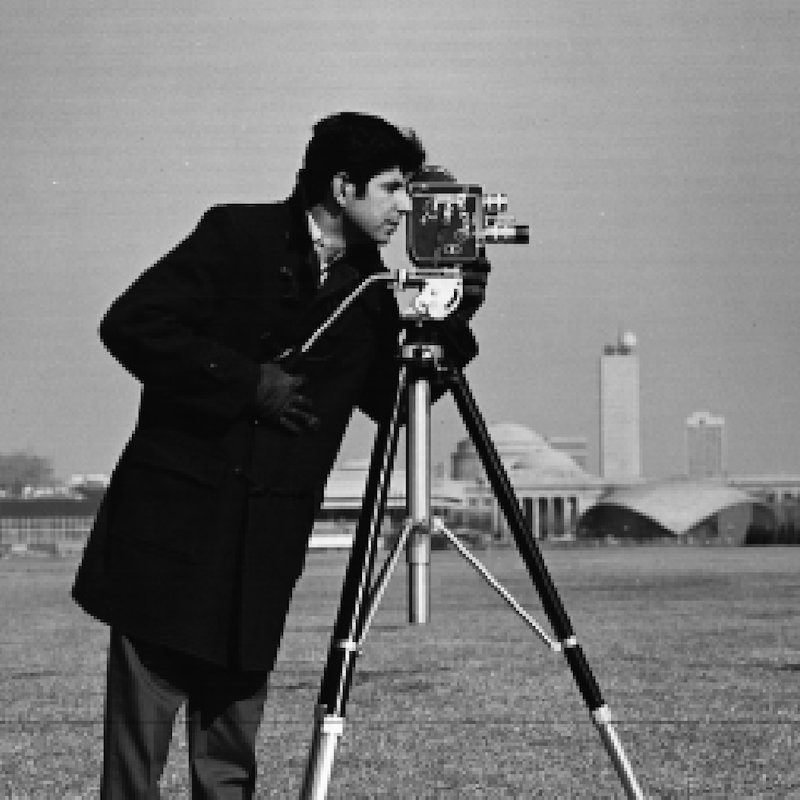
\includegraphics[width=0.4\columnwidth]{images/salt_pepper_origin.jpg}
  %  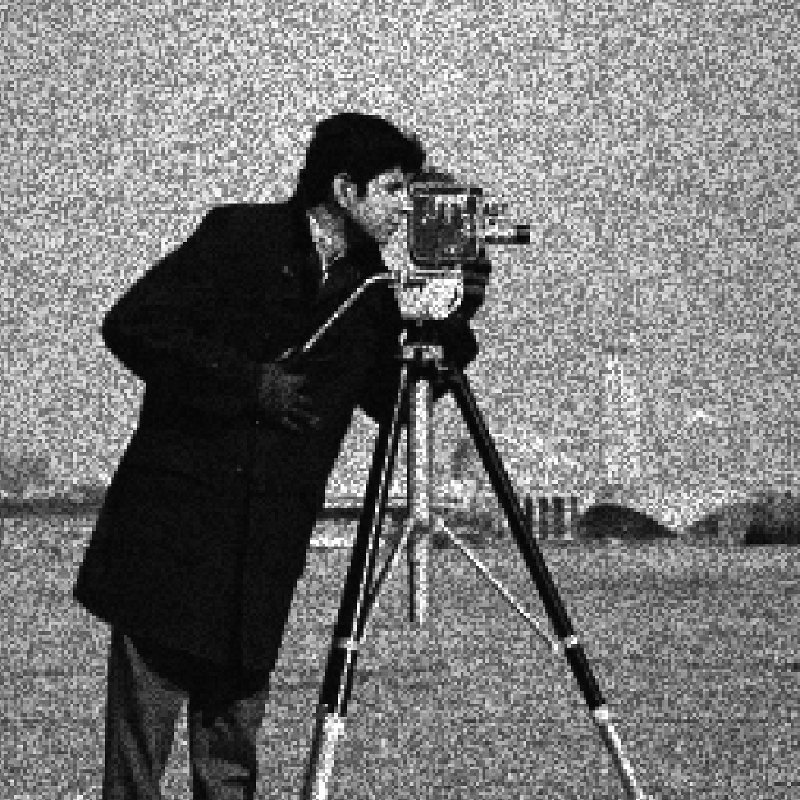
\includegraphics[width=0.4\columnwidth]{images/speckle_noise.jpg}
   
   % Original image (left column) and image corrupted with speckle noise (right column).
%\end{center}

%\end{frame}

%\subsection{Quality of Camera(1)}
%\begin{frame}{Quality of Camera(1)}
%\textbf{Cause of noise images has two reasons :}
%\begin{itemize}
%	\item Weather and Environment
%	\item Quality of camera
%\end{itemize}
%\vspace{0.5cm}
%\textbf{So camera solves 3 problems as below :}

%\begin{center}
%	\begin{itemize}
%		\item Increases with the light
		
		%$\Rightarrow$ Grain shows up more against darker subjects or backgrounds.
		%\item Sensor Size
		
		%$\Rightarrow$Cameras with larger sensors, noise of images will be limited to low.
		%\item Exposure Time 
		
		%$\Rightarrow$ Long exposures can introduce static, which can also be a cause of digital noise.
	%\end{itemize}
%\end{center}

%\end{frame}


\subsection{Solution}

\begin{frame}{Solution}
%\textbf{Definition}

%\vspace{0.5cm}
\textbf{Spatial Filtering :}
\begin{itemize}
\vspace{0.3cm}

\item Median Filter

\

\item Average Filter

\

\item Gaussian Filter
\end{itemize}	
\vspace{1cm}
	
	
	
\textbf{Frequency Domain Filtering :}
\begin{itemize}
\vspace{0.3cm}

\item Wiener Filter
\end{itemize}
\end{frame}



\subsection{Median Filter}
\begin{frame}{Median Filter}

A nonlinear digital filtering technique, often used to remove noise from an image or signal.




%\vspace{2cm}
\begin{center}
		\begin{tabular}{|c|c|c|c|c|}
		\hline 
		234 & 147 & 225 & 214 & 134 \\ 
		\hline 
		231 & \textcolor{blue}{123} & \textcolor{blue}{121} & \textcolor{blue}{223} & 189 \\ 
		\hline 
		124 & \textcolor{blue}{223} & \textcolor{red}{156} & \textcolor{blue}{178} & 196 \\ 
		\hline 
		219 & \textcolor{blue}{125} & \textcolor{blue}{211} & \textcolor{blue}{178} & 124 \\ 
		\hline 
		210 & 185 & 221 & 189 & 134 \\ 
		\hline 
		\end{tabular}
	\end{center}

	\begin{center}
		\begin{tabular}{|c|c|c|c|c|}
		\hline 
		\textcolor{white}{234} & \textcolor{white}{234} & \textcolor{white}{234} & \textcolor{white}{234} & \textcolor{white}{234} \\ 
		\hline 
		\textcolor{white}{234} & \textcolor{white}{234} & \textcolor{white}{234} & \textcolor{white}{234} & \textcolor{white}{234} \\ 
		\hline 
		\textcolor{white}{234} & \textcolor{white}{223} & \textcolor{red}{178} & \textcolor{white}{178} & \textcolor{white}{234} \\ 
		\hline 
		\textcolor{white}{234} & \textcolor{white}{234} & \textcolor{white}{234} & \textcolor{white}{234} & \textcolor{white}{234} \\ 
		\hline 
		\textcolor{white}{234} & \textcolor{white}{234} & \textcolor{white}{234} & \textcolor{white}{234} & \textcolor{white}{234} \\ 
		\hline 
		\end{tabular}
\vspace{0.5cm}

\textbf{Example of median computation}
	\end{center}

\end{frame}

\subsection{Average Filter}
\begin{frame}{Average Filter}
Simply to replace each pixel value in an image with the average value of its neighbors, including itself.

\begin{center}
$k(u,v) = \frac{1}{M}\displaystyle\sum_{(p,q) \in N} i(p,q)$
\end{center}
\vspace{0.5cm}
%Where $k(u,v)$ is new pixel value at position $(u,v)$ of the image, $N$ is neighborhood size, $M$ is total number of pixels in the neighborhood $N$, $i(p,q)$ are original pixel values of the image in the neighborhood $N$. 


\begin{center}


	Filter 3$\times$3
	
	$\dfrac{1}{9}\begin{tabular}{|c|c|c|}
	\hline 
	1 & 1 & 1 \\ 
	\hline 
	1 & 1 & 1 \\ 
	\hline 
	1 & 1 & 1 \\ 
	\hline 
	\end{tabular}$ 	
\end{center}





\end{frame}

\subsection{Average Filter(1)}
\begin{frame}{Average Filter(1)}
\begin{center}
	Filter 5$\times$5
	
	$\dfrac{1}{25}\begin{tabular}{|c|c|c|c|c|}
	\hline 
	1 & 1 & 1 & 1 & 1 \\ 
	\hline 
	1 & 1 & 1 & 1 & 1 \\ 
	\hline 
	1 & 1 & 1 & 1 & 1 \\ 
	\hline 
	1 & 1 & 1 & 1 & 1 \\ 
	\hline 
	1 & 1 & 1 & 1 & 1 \\ 
	\hline 
	\end{tabular} $
\end{center}





\begin{center}
	Filter 7$\times$7
	
	$\dfrac{1}{49}\begin{tabular}{|c|c|c|c|c|c|c|}
	\hline 
	1 & 1 & 1 & 1 & 1 & 1 & 1 \\ 
	\hline 
	1 & 1 & 1 & 1 & 1 & 1 & 1 \\ 
	\hline 
	1 & 1 & 1 & 1 & 1 & 1 & 1 \\ 
	\hline 
	1 & 1 & 1 & 1 & 1 & 1 & 1 \\ 
	\hline 
	1 & 1 & 1 & 1 & 1 & 1 & 1 \\ 
	\hline 
	1 & 1 & 1 & 1 & 1 & 1 & 1 \\ 
	\hline 
	1 & 1 & 1 & 1 & 1 & 1 & 1 \\ 
	\hline 
	\end{tabular} $
\vspace{0.3cm}

\textbf{Example of Average Filter}
\end{center}


\end{frame}

\subsection{Gaussian Filter}
\begin{frame}{Gaussian Filter}
%Gaussian filters are ideal to start experimenting with filtering because their design can be controlled by manipulating just one variable- the variance.
2-D convolution operator that is used to 'blur' images and remove detail and noise.
%In electronics and signal processing, a Gaussian filter is a filter whose impulse response is a Gaussian function (or an approximation to it).
\vspace{0.8cm}

The Gaussian kernel in dimension 2:


%$G(x,y) = \dfrac{1}{2\pi\sigma^2}\exp\left[-\dfrac{(x-\mu_x)^2+(y-\mu_y)^2}{2\sigma^2}\right ]$

%\hspace{3cm}$$\Updownarrow$$

\hspace{3cm}$G(x,y)=\dfrac{1}{2\pi\sigma^2}e^{-{\dfrac{x^2+y^2}{2\sigma^2}}}$\vspace{0.2cm}	

Where $\sigma$ is the standard deviation of the distribution.
\vspace{0.8cm}

Define the Gaussian mask($\sigma$=2):
%$$\mu = 0$$
%$$\sigma = 0.8$$
\begin{center}
	Filter 3$\times$3
	
	$\dfrac{1}{16}\begin{tabular}{|c|c|c|}
	\hline 
	1 & 2 & 1 \\ 
	\hline 
	2 & 4 & 2 \\ 
	\hline 
	1 & 2 & 1 \\ 
	\hline 
	\end{tabular} $
\end{center}
\end{frame}

\subsection{Gaussian Filter(1)}
\begin{frame}{Gaussian Filter(1)}
\begin{center}
	Filter 5$\times$5
	
	$\dfrac{1}{273}\begin{tabular}{|c|c|c|c|c|}
	\hline 
	1 & 4 & 7 & 4 & 1 \\ 
	\hline 
	4 & 16 & 26 & 16 & 4 \\ 
	\hline 
	7 & 26 & 41 & 26 & 7 \\ 
	\hline 
	4 & 16 & 26 & 16 & 4 \\ 
	\hline 
	1 & 4 & 7 & 4 & 1 \\ 
	\hline 
	\end{tabular}$ 
\end{center}

\begin{center}
	Filter 7$\times$7
	
	$\dfrac{1}{1003}$\begin{tabular}{|c|c|c|c|c|c|c|}
		\hline 
		0 & 0 & 1 & 2 & 1 & 0 & 0 \\ 
		\hline 
		0 & 3 & 13 & 22 & 13 & 3 & 0 \\ 
		\hline 
		1 & 13 & 59 & 97 & 59 & 13 & 1 \\ 
		\hline 
		2 & 22 & 97 & 159 & 97 & 22 & 2 \\ 
		\hline 
		1 & 13 & 59 & 97 & 59 & 13 & 1 \\ 
		\hline 
		0 & 3 & 13 & 22 & 13 & 3 & 0 \\ 
		\hline 
		0 & 0 & 1 & 2 & 1 & 0 & 0 \\ 
		\hline 
	\end{tabular} 
\end{center}
\end{frame}

\subsection{Wiener Filter}
\begin{frame}{Wiener Filter}
%The Wiener filtering is optimal in terms of the mean square error. In other words, it minimizes the overall mean square error in the process of inverse filtering and noise smoothing.

Weiner filter is a frequency-domain method for image denosing. %Wiener filter removes noise from an image signal by minimizing mean square error between the original noiseless image signal and the received image signal.
%
%The Wiener filter is a filter used to produce an estimate of a desired or target random process by linear time-invariant (LTI) filtering of an observed noisy process, assuming known stationary signal and noise spectra, and additive noise.
\vspace{1cm}
\begin{itemize}
	\item Assumption %: signal and (additive) noise are stationary linear stochastic processes with known spectral characteristics or known autocorrelation and cross-correlation
	\item Requirement %: the filter must be physically realizable/causal (this requirement can be dropped, resulting in a non-causal solution)
	\item Performance criterion %: minimum mean-square error (MMSE)
\end{itemize}

%\textbf{What is stationary linear filter meaning ?}


\end{frame}
%\subsection{Wiener Filter(1)}
%\begin{frame}{Wiener Filter(1)}
%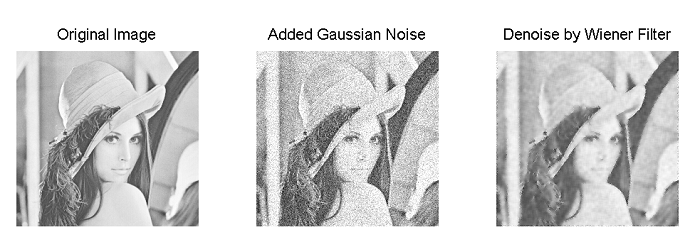
\includegraphics{Wiener.png}



%Weiner filter are characterized by following:
%\vspace{0.5cm}
%\begin{itemize}
%	\item \textbf{Assumption:}
	
%	Stationary linear with known spectral characteristics or
%	known autocorrelation and cross-correlation.
	
	
%	\
	
%	\item \textbf{Requirement:}
	
%	The filter must be physically feasible 
	 
	
%	\
	
%	\item \textbf{Performance criterion:} 
	
%	Minimum mean square error.
	
%\end{itemize} 


%\end{frame}





\subsection{Evaluation}
\begin{frame}{Evaluation}

\

%A measure of the quality of an estimator—it is always non-negative, and values closer to zero are better.
Mean Squared Error :
\begin{center}

\vspace{0.8cm}

	    MSE = $\frac{1}{mn}{\sum_{i=1}^{m}\sum_{j=1}^{n}(f'_{ij}-f_{ij})^2}$ 
	%\end{equation}
\end{center}
\vspace{1cm}

Peak Signal To Noise Ratio : 
\begin{center}

\vspace{0.8cm}

$PSNR = 10 \log_{10}\frac{R^2}{MSE}$
\end{center}
 

\end{frame}




\subsection{Results and Discussion
}
\begin{frame}{Results and Discussion
}
\begin{center}


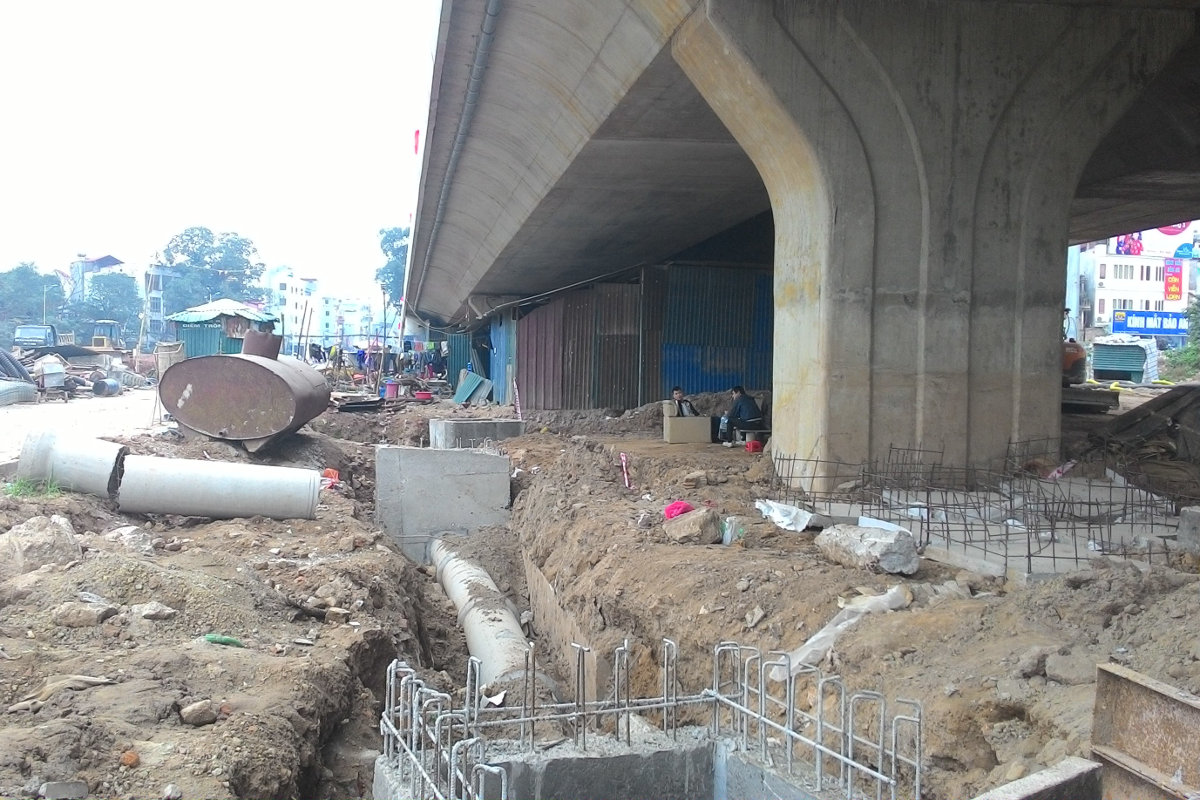
\includegraphics[width=0.27\linewidth]{images/example-construction.jpg}
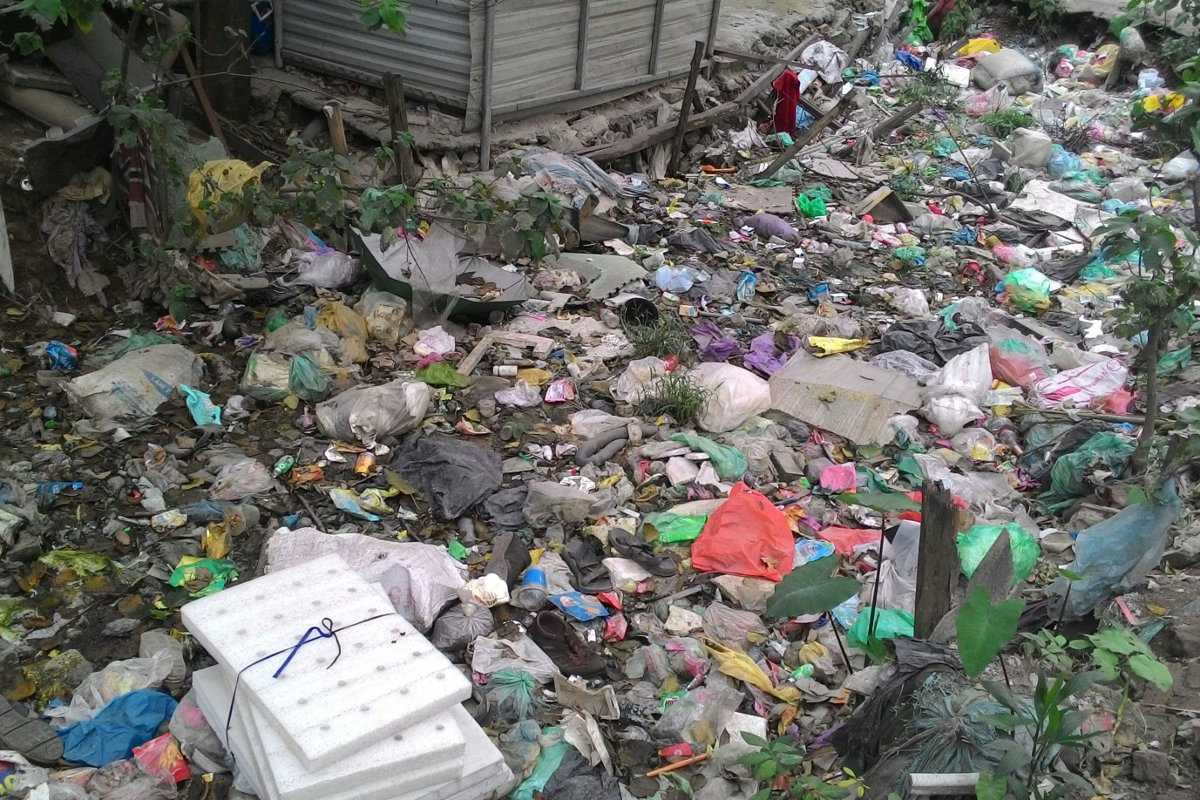
\includegraphics[width=0.27\linewidth]{images/example-rubbish.jpg}
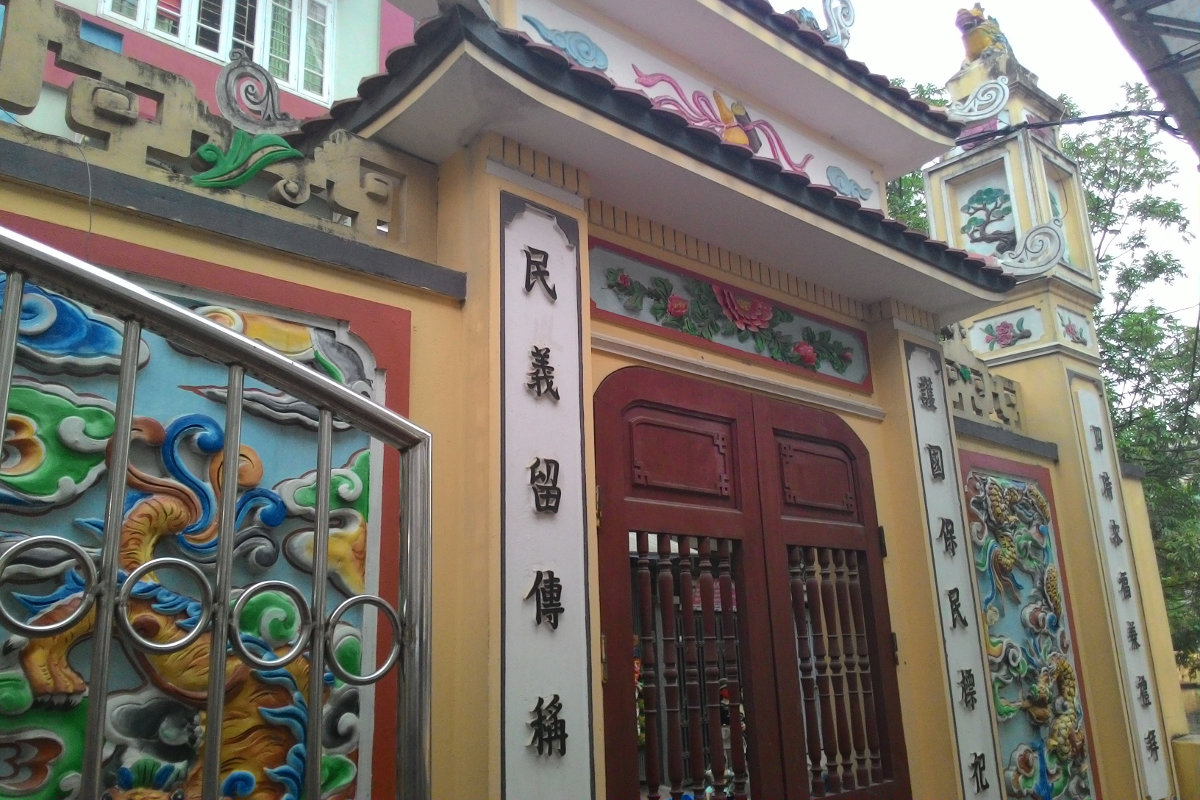
\includegraphics[width=0.27\linewidth]{images/example-pagoda.jpg}
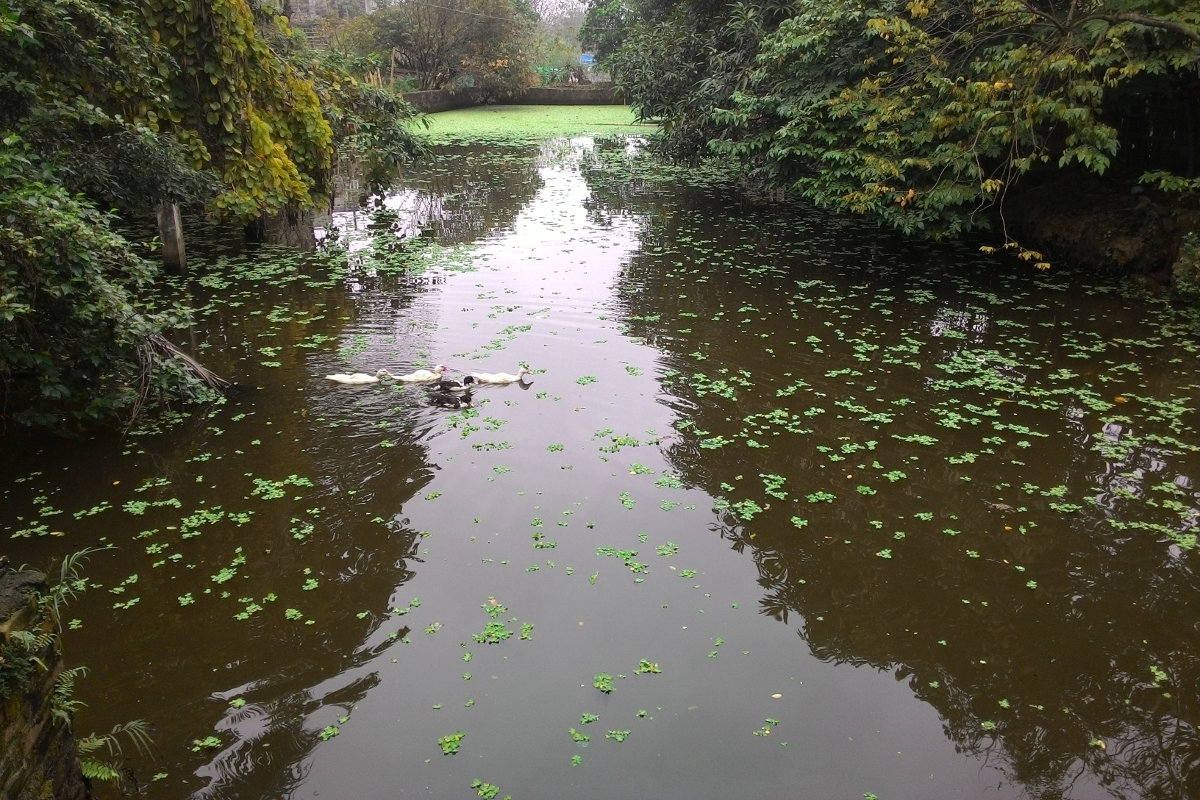
\includegraphics[width=0.27\linewidth]{images/example-pond.jpg}
	



\textbf{SWARMS project dataset}
\end{center}
\end{frame}

\subsection{Construction Sites}
\begin{frame}{Construction Sites}
\begin{figure}[h]
	\centering
	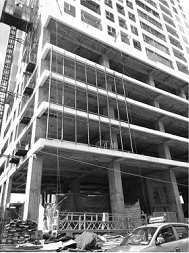
\includegraphics[width=0.18\columnwidth]{images/construction1.jpg}
	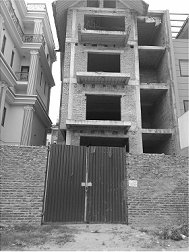
\includegraphics[width=0.18\columnwidth]{images/construction2.jpg}
	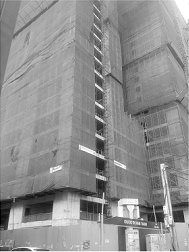
\includegraphics[width=0.18\columnwidth]{images/construction3.jpg}
	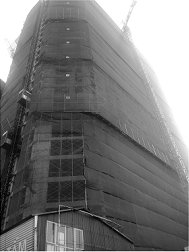
\includegraphics[width=0.18\columnwidth]{images/construction4.jpg}
	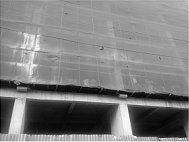
\includegraphics[width=0.18\columnwidth]{images/construction5.jpg}
	\caption{Evaluated construction site photos. From left to right: construction1, construction2, construction3, construction4, construction5}
	\label{fig:construction}
\end{figure}
\end{frame}

\subsection{Evaluated metrics for construction site photos
}
\begin{frame}{Evaluated metrics for construction site photos
}
\begin{center}
%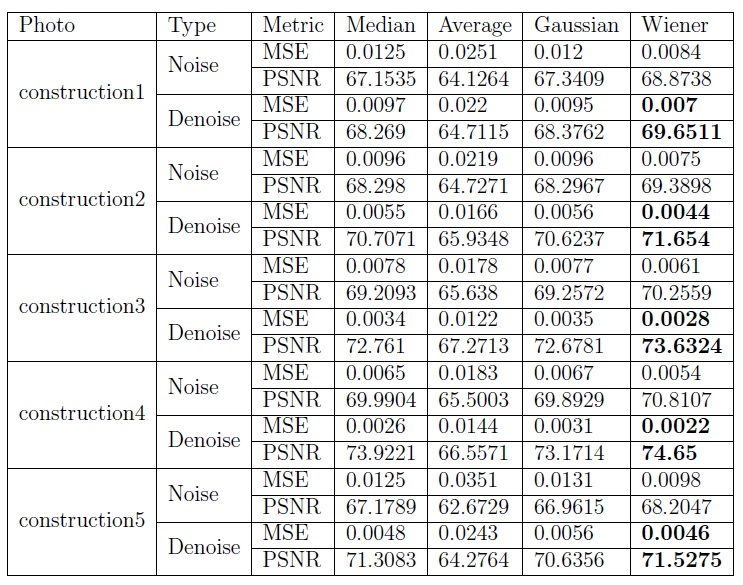
\includegraphics{con1.jpg}
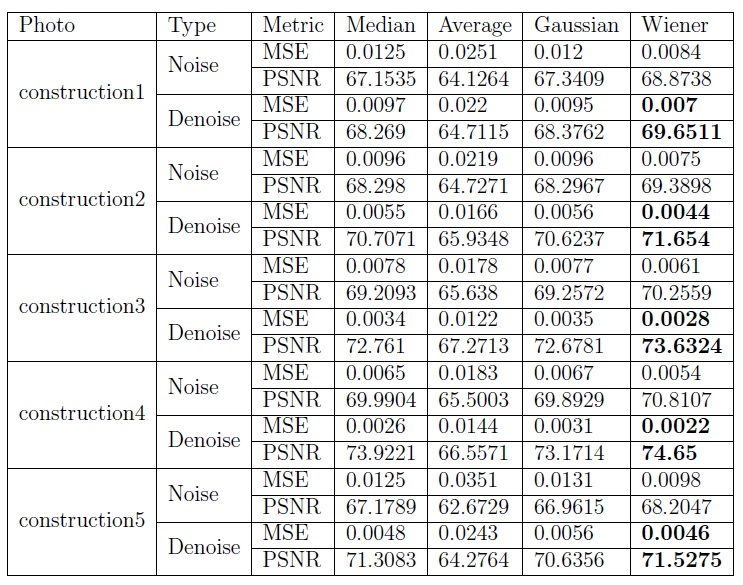
\includegraphics[width=10cm,height=7cm]{con1.jpg}

\end{center}
\end{frame}





\subsection{Rubbish}
\begin{frame}{Rubbish}
\begin{figure}[h]
	\centering
	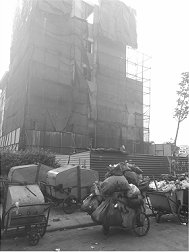
\includegraphics[width=0.18\columnwidth]{images/rubbish1.jpg}
	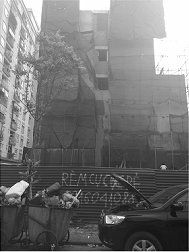
\includegraphics[width=0.18\columnwidth]{images/rubbish2.jpg}
	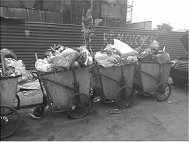
\includegraphics[width=0.18\columnwidth]{images/rubbish3.jpg}
	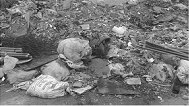
\includegraphics[width=0.18\columnwidth]{images/rubbish4.jpg}
	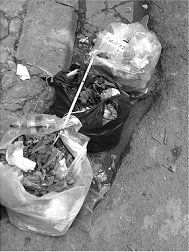
\includegraphics[width=0.18\columnwidth]{images/rubbish5.jpg}
	\caption{Evaluated rubbish photos. From left to right: rubbish1, rubbish2, rubbish3, rubbish4, rubbish5}
	\label{fig:rubbish}
\end{figure}


\end{frame}


\subsection{Evaluated metrics for rubbish photos}
\begin{frame}{Evaluated metrics for rubbish photos}
\begin{center}
%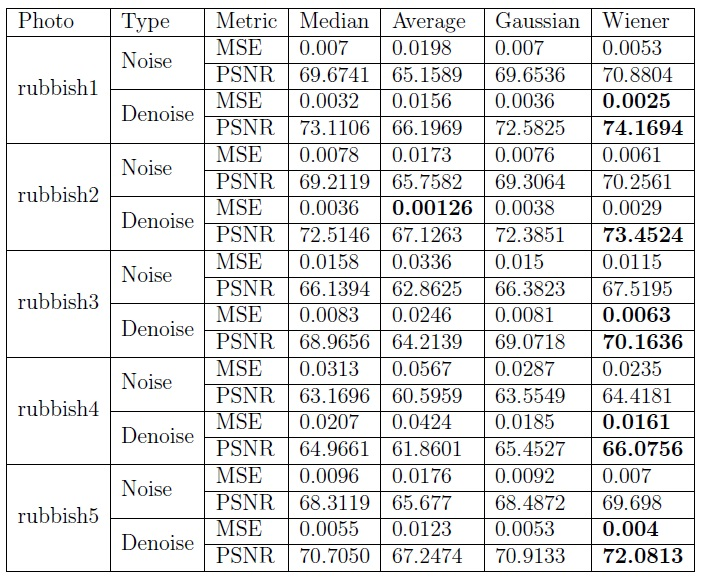
\includegraphics{rub1.jpg}
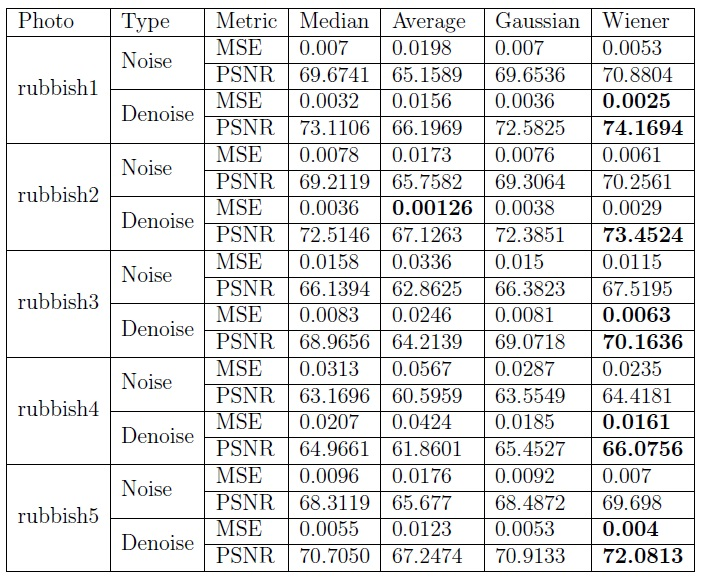
\includegraphics[width=10cm,height=7cm]{rub1.jpg}
\end{center}


\end{frame}





\subsection{Pagoda}
\begin{frame}{Pagoda}
\begin{figure}[h]
	\centering
	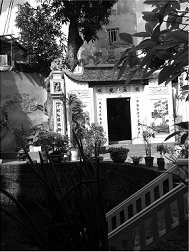
\includegraphics[width=0.18\columnwidth]{images/pagoda1.jpg}
	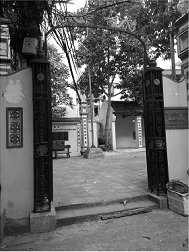
\includegraphics[width=0.18\columnwidth]{images/pagoda2.jpg}
	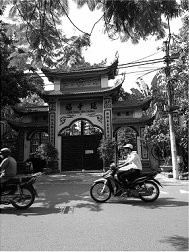
\includegraphics[width=0.18\columnwidth]{images/pagoda3.jpg}
	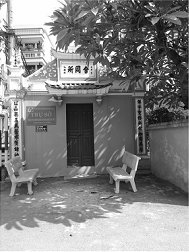
\includegraphics[width=0.18\columnwidth]{images/pagoda4.jpg}
	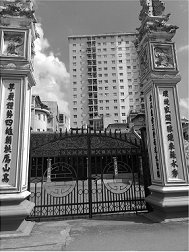
\includegraphics[width=0.18\columnwidth]{images/pagoda5.jpg}
	\caption{Evaluated pagoda photos. From left to right: pagoda1, pagoda2, pagoda3, pagoda4, pagoda5}
	\label{fig:pagoda}
\end{figure}
\end{frame}

\subsection{Evaluated metrics for pagoda photos
}
\begin{frame}{Evaluated metrics for pagoda photos
}
\begin{center}
%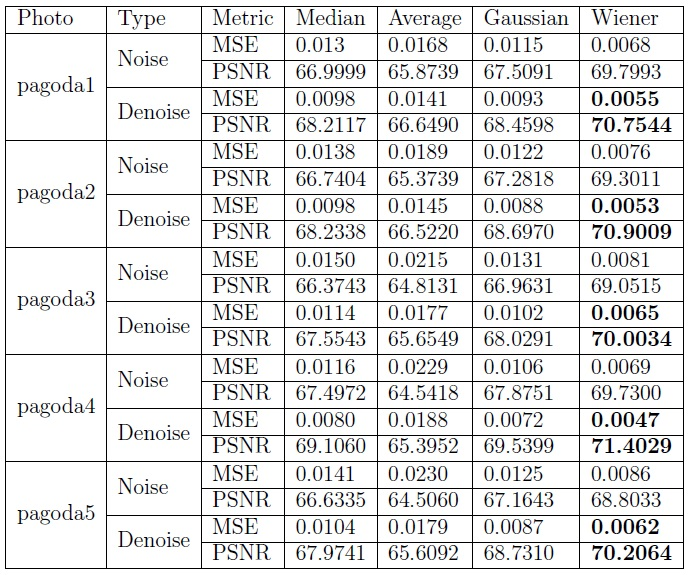
\includegraphics{pag1.jpg}
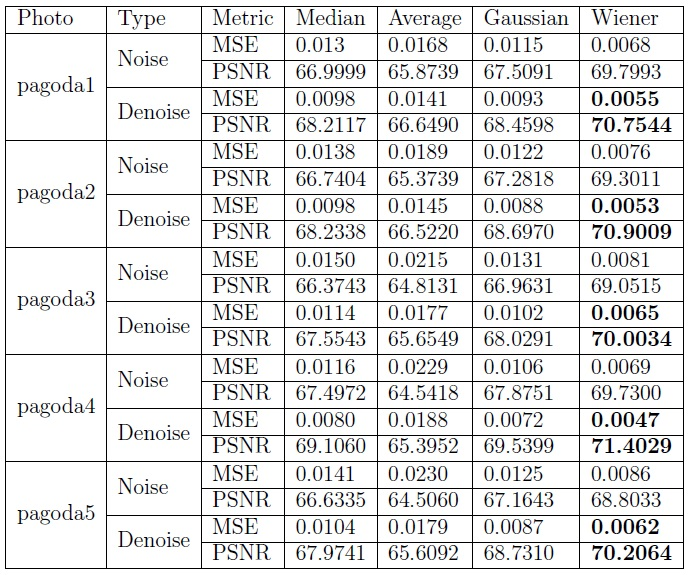
\includegraphics[width=10cm,height=7cm]{pag1.jpg}
\end{center}
\end{frame}







\subsection{Pond}
\begin{frame}{Pond}
\begin{center}
\begin{figure}[h]
	\centering
	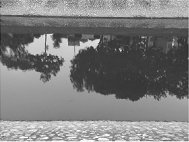
\includegraphics[width=0.18\columnwidth]{images/pond1.jpg}
	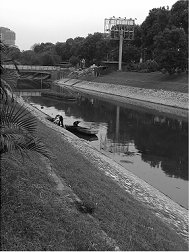
\includegraphics[width=0.18\columnwidth]{images/pond2.jpg}
	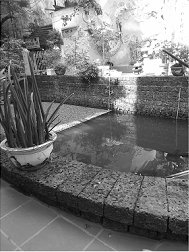
\includegraphics[width=0.18\columnwidth]{images/pond3.jpg}
	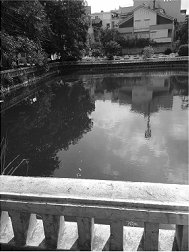
\includegraphics[width=0.18\columnwidth]{images/pond4.jpg}
	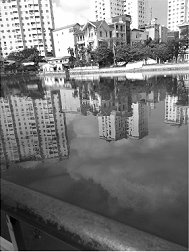
\includegraphics[width=0.18\columnwidth]{images/pond5.jpg}
	\caption{Evaluated pond photos. From left to right: pond1, pond2, pond3, pond4, pond5}
	\label{fig:pond}
\end{figure}


\end{center}
\end{frame}


\subsection{Evaluated metrics for pond photos}
\begin{frame}{Evaluated metrics for pond photos}
\begin{center}
%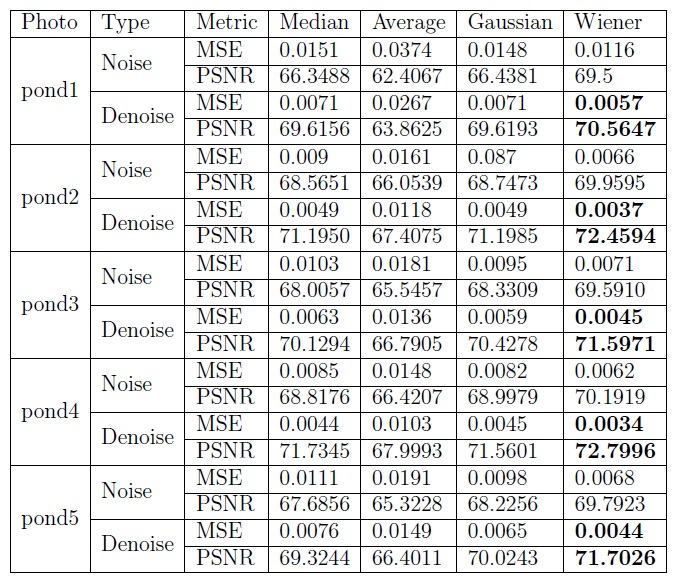
\includegraphics{pon1.jpg}
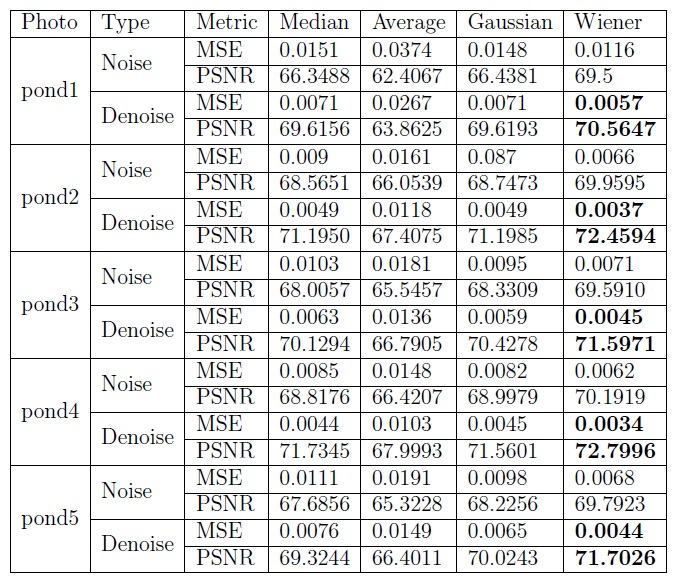
\includegraphics[width=10cm,height=7cm]{pon1.jpg}
\end{center}
\end{frame}

\subsection{Discussion}
\begin{frame}{Discussion}
\begin{center}
	\begin{tabular}{| l | l | l | l | l |}
		\hline
		Photo 			& Median 	& Average 	& Gaussian 	& Weiner 	\\ \hline
		construction1	& 9.762		& 3.038		& 2.161		& 15.524	\\ \hline
		rubbish1		& 9.145		& 3.187		& 2.158		& 11.795	\\ \hline
		pagoda1			& 8.909		& 2.998		& 2.170		& 12.372	\\ \hline
		pond1			& 7.543		& 2.68		& 1.826		& 7.329		\\ \hline
	\end{tabular}



\textbf{Method runtimes (in milliseconds)}

\end{center}
\end{frame}






\subsection{Conclusion}
\begin{frame}{Conclusion}
\begin{center}
\begin{itemize}
	\item The best of results
	
	 Wiener filter with  MSE is minimum mean square error and it is maximum PSNR.
	
	\ 
	
	\item  Disadvantage 
	
	At all method, this method has runtimes which is the longest .

	
	\
    
    \item Future development
     
      Improvement of the proposed method over the existing approaches in terms of visual quality.
\end{itemize}
\end{center}
 

\end{frame}



\subsection{}
\begin{frame}{}

\begin{center}
	\begin{LARGE}
		THANK YOU !!!
	\end{LARGE} 
\end{center}
\end{frame}








\end{document}
